\documentclass[a4paper,12pt]{article}
\usepackage[utf8]{inputenc}
\usepackage[T1]{fontenc}
\usepackage[ngerman]{babel}
\usepackage{geometry}
% Anpassung der Ränder und des Header-Platzes, um fancyhdr-Warnungen zu vermeiden
\geometry{a4paper, left=2.5cm, right=2.5cm, top=3cm, bottom=3cm, headheight=15pt}
\usepackage{fancyhdr}
\usepackage{hyperref}
\usepackage{url}
\usepackage{listings}
\usepackage[dvipsnames]{xcolor}
\usepackage{pdfpages}
\usepackage{graphicx}


\lstset{
   literate={ö}{{\"o}}1
           {ä}{{\"a}}1
           {ü}{{\"u}}1
           {ß}{{\ss}}1
           {é}{{\'e}}1,
   inputencoding=ansinew,
   extendedchars=true,
   basicstyle=\scriptsize\ttfamily,
   numberstyle=\scriptsize,
   breaklines=true,
   tabsize=4,
   numbersep=5pt
}
\lstdefinestyle{textstyle}{
    language={},                 % Verhindert blau markierte Wörter im Text
    basicstyle=\small\sffamily,  % Serifenlose Schrift (Arial-Look)
    breaklines=true,             % Automatischer Zeilenumbruch
    xleftmargin=0pt,             % Absolut keine Einrückung von links
    xrightmargin=0pt,            % Nutzt die volle Breite rechts
    frame=none,                  % Kein Kasten drumherum
    numbers=none,                % Keine Zeilennummern
    keepspaces=true,             % Behält deine Leerzeichen/Formatierung bei
    columns=fullflexible,        % WICHTIG: Erlaubt "normale" Buchstabenabstände
    literate={ä}{{\"a}}1 {ö}{{\"o}}1 {ü}{{\"u}}1 {ß}{{\ss}}1 % Fix für Umlaute
}

\lstdefinestyle{customcpp}{
   language=C++,
   frame=single,
   numbers=left,
   keywordstyle=\color{blue}\bfseries,
   stringstyle=\color{BrickRed}\ttfamily,
   commentstyle=\color{OliveGreen}\ttfamily,
   showspaces=false,
   showstringspaces=false,
   showtabs=false,
   xleftmargin=5px
}

% Setup für Kopf- und Fußzeilen gemäß Vorlage
\pagestyle{fancy}
\fancyhf{} % Löscht Standard-Kopf-/Fußzeilen
\lhead{J. Rieger, L. Kieweg}
\chead{Systemdokumentation}
\rhead{Seite \thepage}
\renewcommand{\headrulewidth}{0.4pt}
\renewcommand{\footrulewidth}{0pt}

\begin{document}

%****************** self defined commands ***************************
%include a .cpp source file
%usage: \cppfile{../path_to_your_file/filename}
\newcommand{\cppfile}[1]{
\begin{itemize}
\item[]\lstinputlisting[label={lst:\detokenize{#1}}, style=customcpp,
    caption=\texttt{\detokenize{#1.cpp}}]{#1.cpp}
\end{itemize}
}

%include a .h source file
%usage: \hfile{../path_to_your_file/filename}
\newcommand{\hfile}[1]{
\begin{itemize}
\item[]\lstinputlisting[label={lst:\detokenize{#1}}, style=customcpp,
    caption=\texttt{\detokenize{#1.h}}
]{#1.h}
\end{itemize}
}

%include a module (.cpp and .h)
%usage: \hfile{../path_to_your_file/filename}
\newcommand{\cppmodul}[1]{
\begin{itemize}
\item[]\lstinputlisting[caption=#1.h,label="lst:#1-header", style=customcpp]{#1.h}
\item[]\lstinputlisting[caption=#1.cpp,label="lst:#1-impl", style=customcpp]{#1.cpp}
\end{itemize}
}

%include a code snippet
%usage: \hfile{../path_to_your_file/filename}{startline}{endline}
\newcommand{\snippet}[3]{
\begin{itemize}
\item[]\lstinputlisting[caption=#1.cpp,label="lst:#1-snip", style=customcpp, firstline=#2,lastline=#3]{#1.cpp}
\end{itemize}
}

%include a test-output file 
%usage: \testoutput{../path_to_your_file/filename}
\newcommand{\testoutput}[1]{
\begin{itemize}
\item[]\lstinputlisting[caption=#1]{#1.txt}
\end{itemize}
}

%include a figure -> ensure that the picture is in the pics directory
%usage: \fig{name_of_picture}{width}{caption text}
%width between 0.0 - 1.0 -> correspond with textwidth
\newcommand{\fig}[3]{
\begin{figure}[H]
\centering
\includegraphics[width=#2\textwidth]{pics/#1.PNG}
\caption{#3}
\label{fig:#1}
\end{figure}
}

\lstset{
   literate={ö}{{\"o}}1
           {ä}{{\"a}}1
           {ü}{{\"u}}1
           {ß}{{\ss}}1
           {é}{{\'e}}1,
   inputencoding=ansinew,
   extendedchars=true,
   basicstyle=\scriptsize\ttfamily,
   numberstyle=\scriptsize,
   breaklines=true,
   tabsize=4,
   numbersep=5pt
}

\lstdefinestyle{customcpp}{
   language=C++,
   frame=single,
   %backgroundcolor=\color{mygray},
   numbers=left,
   keywordstyle=\color{blue}\bfseries,
   stringstyle=\color{BrickRed}\ttfamily,
   commentstyle=\color{OliveGreen}\ttfamily,
   showspaces=false,
   showstringspaces=false,
   showtabs=false,
   xleftmargin=5px
}

% Angabe
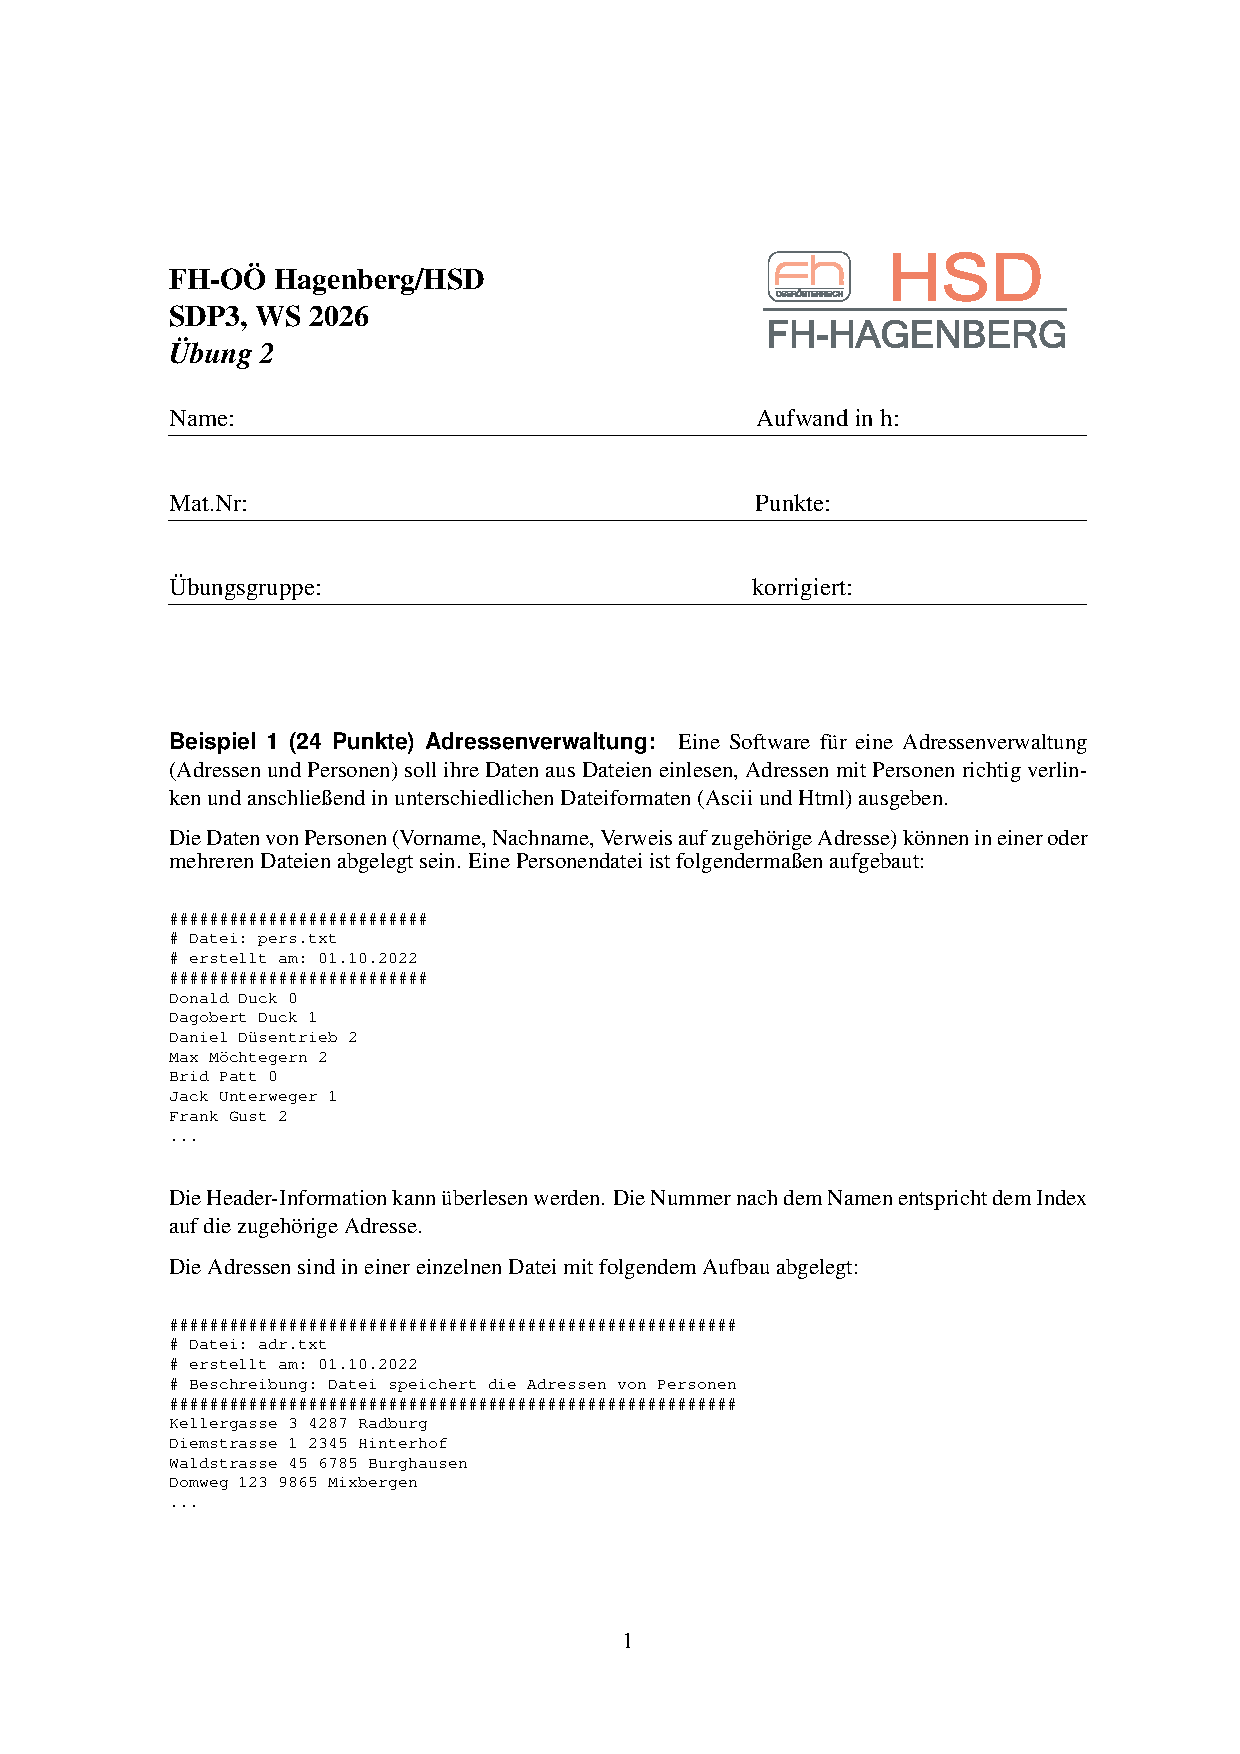
\includepdf[pages=-]{Angabe.pdf}



% -- Titelseite --
\begin{titlepage}
\vspace*{-1cm}
\noindent
HSD\\
OBERÖSTERREICH\\
FH-HAGENBERG

\vspace{4cm}
\begin{center}
{\Huge \textbf{Systemdokumentation}}\\[1cm]
{\Large \textbf{Addressverwaltung}}\\[0.5cm]
{\large Version 1.0}\\[2cm]
{\large J. Rieger, L. Kieweg}\\[0.5cm]
{\large Hagenberg, 21. Oktober 2025}
\end{center}

\vspace{3cm}
\noindent
Dieses Dokument zeigt den prinzipiellen Aufbau einer Systemdokumentation für Software-Projekte. Die einzelnen Kapitel sind mit Kommentaren versehen, welche die Struktur und den Inhalt erläutern.
\end{titlepage}

% -- Inhaltsverzeichnis --
\newpage
\tableofcontents
\newpage

% -- Kapitel 1 --
\section{Organisatorisches}
\subsection {Team}
\begin{itemize}
\item Julian Rieger, Matr.-Nr: S2510306023, E-Mail: S25010306023@fhooe.at
\item Leander Kieweg, Matr.-Nr: S2510306014, E-Mail: S2510306014@fhooe.at
\end{itemize}

\subsection{Aufteilung der Verantwortungsbereiche}
\begin{itemize}
\item Julian Rieger
    \begin{itemize}
        \item Implementierung der Klassen: Address, Person, Reader, AddressReader, PersonReader
        \item Implementierung des Testtreibers
        \item Verfassen der Systemdokumentation
    \end{itemize}
\item Leander Kieweg
    \begin{itemize}
        \item Implementierung der Klassen: AddressManager, HtmlWriter, AsciiWriter, Writer 
        \item Design des Klassendiagrams
        \item Implementierung des Testtreibers

    \end{itemize}
\end{itemize}

\subsection{Aufwand}
\begin{itemize}
\item Julian Rieger: geschätzt: 7h, tatsächlich 8h
\item Leander Kieweg: geschätzt 7h, tatsächlich 8h
\end{itemize}
% -- Kapitel 2 --
\section{Anforderungsdefinition (Systemspezifikation)}
Es wird eine Verwaltungssoftware für eine Adressverwaltung bereitgestellt. Das Programm liest aus seperaten Textdateien die Adressen, sowie die Personen ein, und erstellt intern eine Zuweisung der beiden Daten. Das System beruht auf einem Template Method Pattern und besitzt eine abstrakte übergeordnete Basisklasse 'Object'. Die Addressverwaltung erfolgt ausschließlich durch die Klasse AddressManager, und liefert folgende Funktionalität:
\begin{itemize}
    \item Das Hinzufügen von Adressen durch Auslesen einer Textdatei
    \item Das Hinzufügen von Personen durch Auslesen eienr Textdatei
    \item Das Ausgeben der registrierten Datenpaaren formatiert in HTML- und ASCII-Format.
\end{itemize}
Das Anlegen von Addressen oder Personen wird ausschließlich vom Reader ausgeführt. Das manuelle Manipulieren von den Daten des AddressManager ist nicht möglich bzw. vorgesehen. Für das Lesen und Schreiben verwendet der AddressManager intern ein dediziertes Reader und Writer Objekt, welches diese Funktionalität vollständig übernimmt. Der PersonReader und der AddressReader sind als friend-Klassen beim AddressManager definiert, sodass diese von außen den alleinigen Zugriff auf die Add-Funktionen besitzen.
% -- Kapitel 3 -- 
\section{Systementwurf}
\subsection{Klassendiagram}

\begin{figure}[htbp]
  \centering
  \makebox[\textwidth][c]{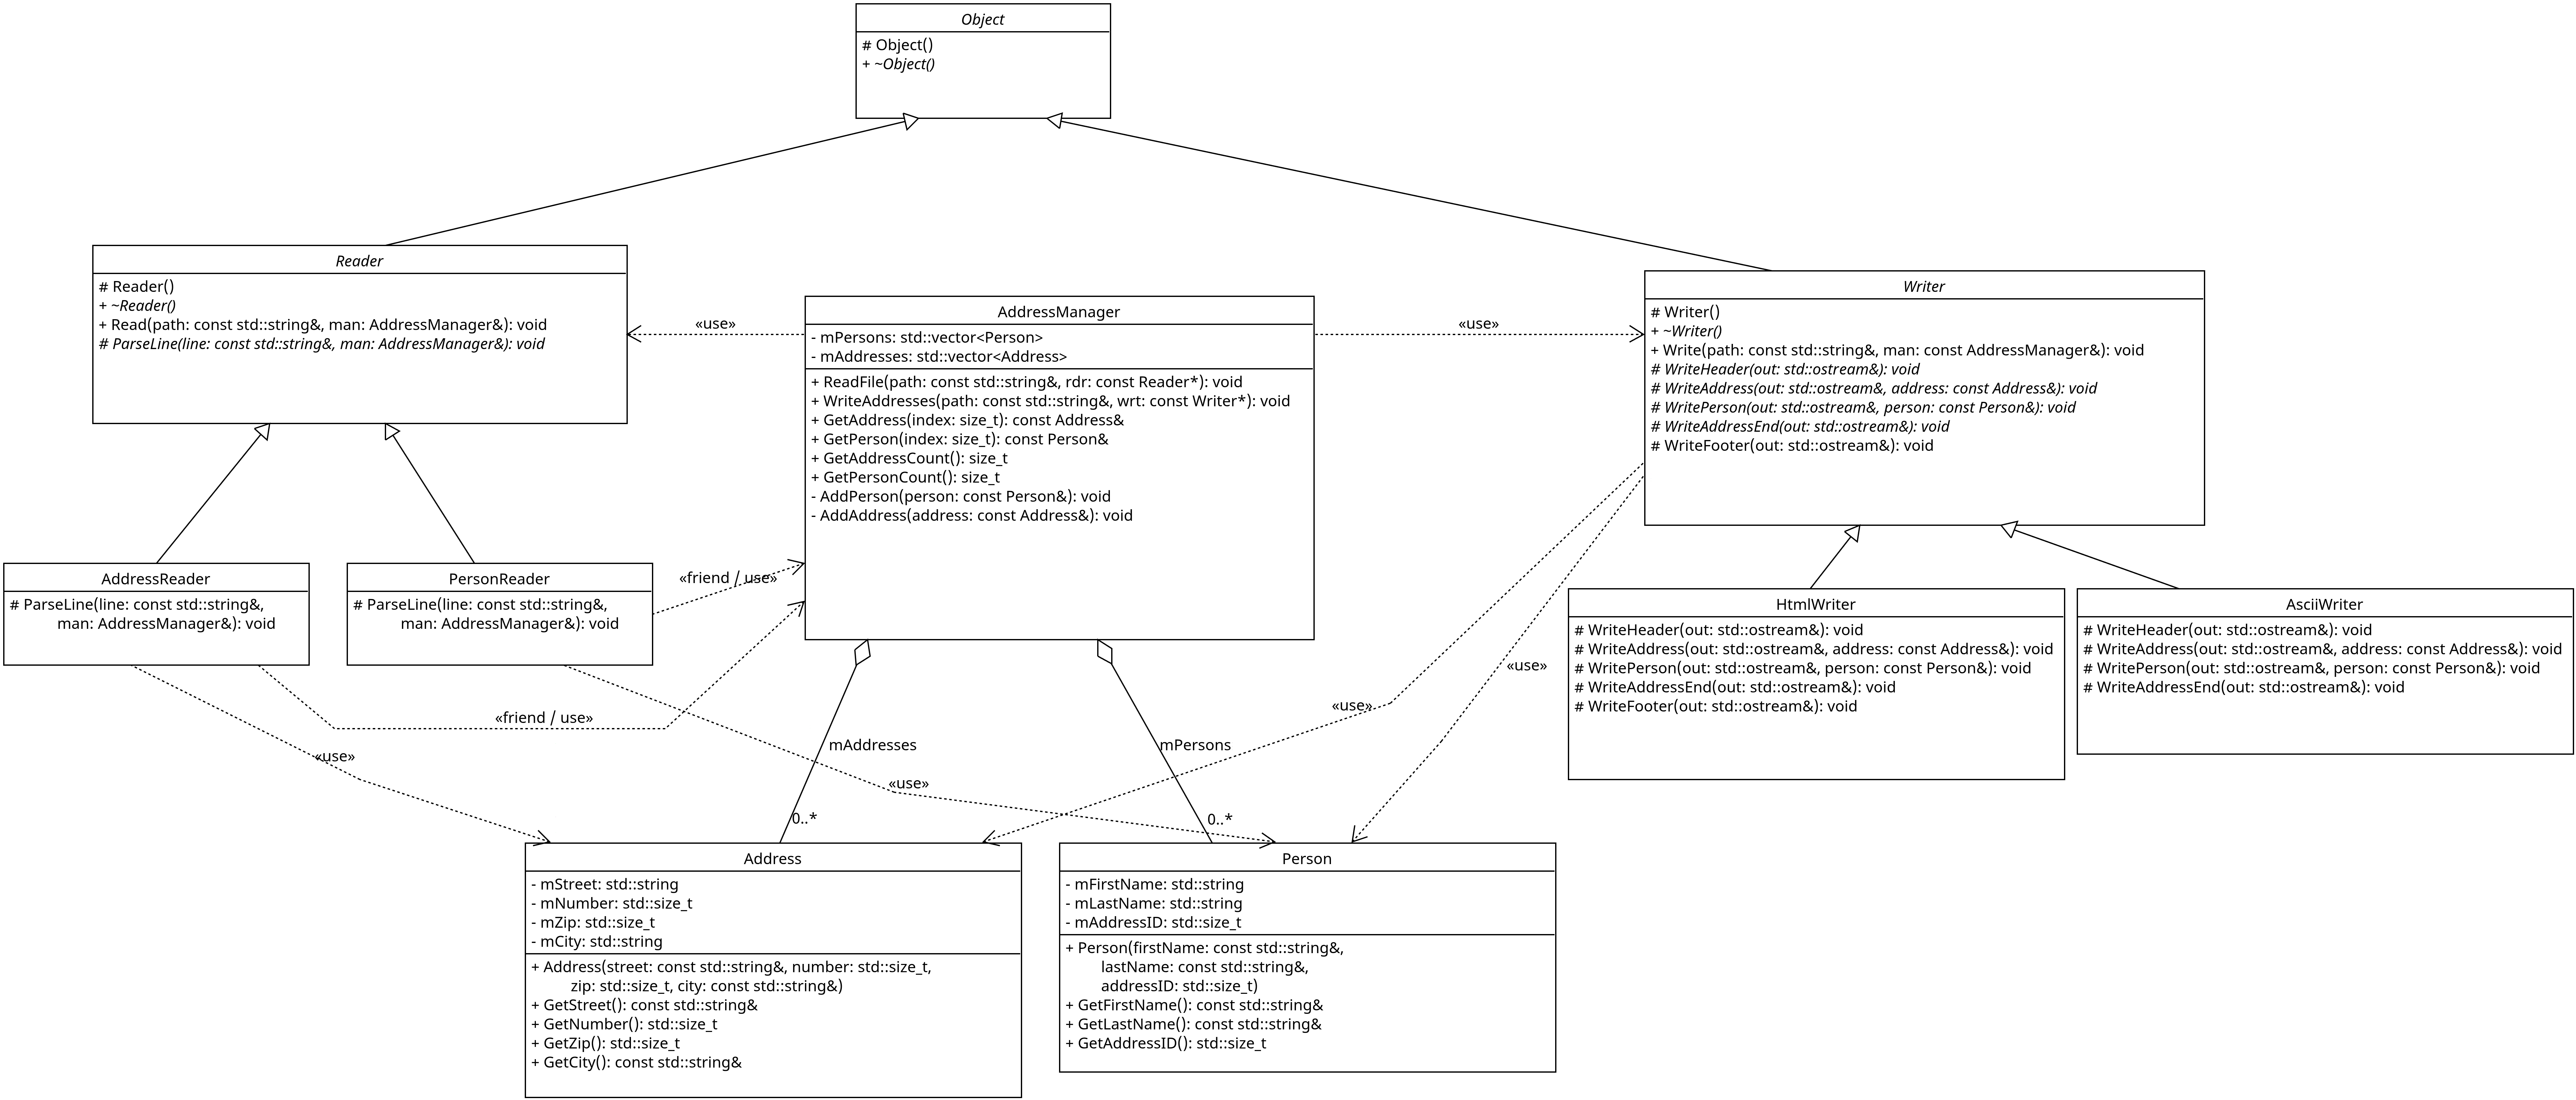
\includegraphics[width=1.25\textwidth]{addressmanager.png}}
  \caption{Klassendiagramm AddressManager}
\end{figure}

Anmerkung: Das Klassendiagram steht für bessere Lesbarkeit ebenfalls im Sysdoku-Ordner zur Verfügung.

\subsection{Designentscheidungen}
Als Design Pattern wurde das Template Method Pattern festgelegt. Es wird für die Reader und Writer Vererbung genutzt, wobei beide auch von Object erben, um den virtual destructor zu gewährleisten. Dazu zählt der AddressReader, PersonReader, HtmlWriter und AsciiWriter. Diese implementieren ihre eigenen ParseLine() bzw. WriteLine() Funktionen, je nach gewünschtem Format. Diese Funktionen sind in den Basisklassen als pure virtual markiert. Die Funktionen Read() und Write() der Basisklassen sind jedoch bereits in den Basisklassen implementiert. Reader und Writer sind beides abstrakte Klassen, d.h. ihre Konstruktoren sind als protected festgelegt, sodass diese nicht von außen zugänglich sind.

% -- Kapitel 4 --
\section{Komponentenentwurf}
Die HTML-Startdatei befindet sich im Verzeichnis ./../doxy/html/index.html
% -- Kapitel 5 --
\section{Testprotokollierung}
\subsection{Ausgabe Konsole Testtreiber}
\begin{lstlisting}[style=textstyle]
[SUCCESS] person and address file are read
[SUCCESS] persons and addresses are stored
[SUCCESS] first person is Donald Duck with address 0
[SUCCESS] first address is Kellergasse 3, 4287 Radburg
[SUCCESS] ascii and html file are written
[SUCCESS] null reader -> invalid_argument
[SUCCESS] null writer -> invalid_argument
[SUCCESS] missing file -> runtime_error
[SUCCESS] wrong line format -> runtime_error
[SUCCESS] wrong address index -> out_of_range
[SUCCESS] wrong person index -> out_of_range
[SUCCESS] person without address -> out_of_range
\end{lstlisting}

\newpage
\subsection{Ascii Output File}
\begin{lstlisting}[style=textstyle]
Adressen mit zugeordneten Personen
----------------------------------
4287 Radburg
Kellergasse 3
    Donald Duck
    Brid Patt

2345 Hinterhof
Diemstrasse 1
    Dagobert Duck
    Jack Unterweger

6785 Burghausen
Waldstrasse 45
    Daniel Düsentrieb
    Max Möchtegern
    Frank Gust

9865 Mixbergen
Domweg 123


\end{lstlisting}
\newpage
\subsection{Html Output File}
\begin{figure}[htbp]
    \centering
    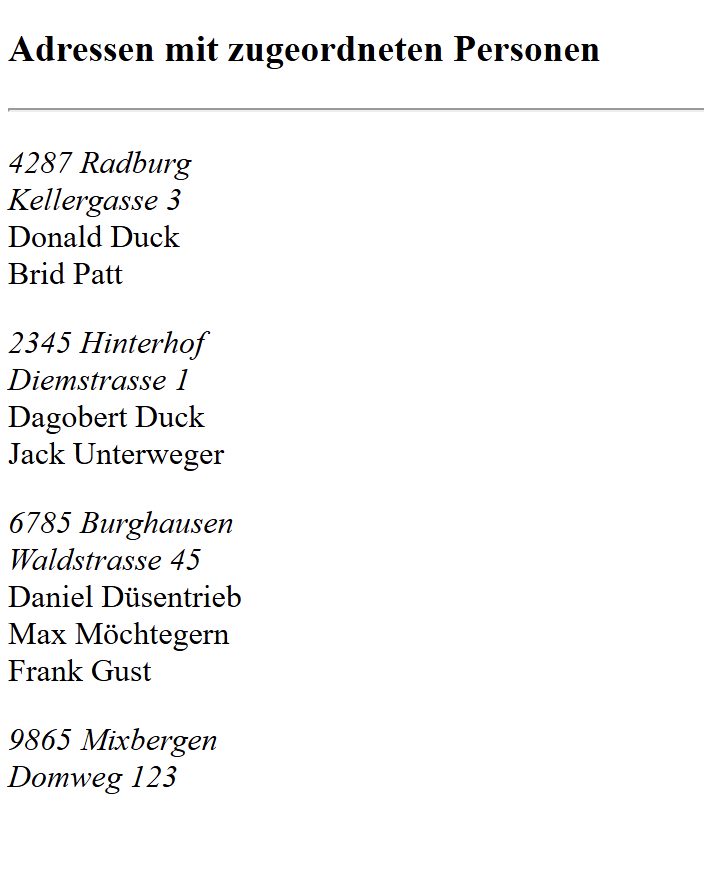
\includegraphics[width=0.8\textwidth]{HtmlOutput.png}
    \caption{HtmlOutput}
    \label{fig:mein_bild}
\end{figure}


% -- Kapitel 6 --
\newpage
\section{Quellcode}
\hfile{../Object}
\cppfile{../Address}
\hfile{../Address}
\cppfile{../Person}
\hfile{../Person}
\cppfile{../Reader}
\hfile{../Reader}
\cppfile{../AddressReader}
\hfile{../AddressReader}
\cppfile{../PersonReader}
\hfile{../PersonReader}
\cppfile{../Writer}
\hfile{../Writer}
\cppfile{../HtmlWriter}
\hfile{../HtmlWriter}
\cppfile{../AsciiWriter}
\hfile{../AsciiWriter}
\cppfile{../AddressManager}
\hfile{../AddressManager}
\cppfile{../main}
\end{document}